\documentclass[12pt, twoside]{article}
\usepackage[letterpaper, margin=1in, headsep=0.5in]{geometry}
\usepackage[english]{babel}
\usepackage[utf8]{inputenc}
\usepackage{amsmath}
\usepackage{amsfonts}
\usepackage{amssymb}
\usepackage{tikz}
%\usetikzlibrary{quotes, angles}

\usepackage{graphicx}
\usepackage{enumitem}
\usepackage{multicol}

\usepackage{fancyhdr}
\pagestyle{fancy}
\fancyhf{}
\renewcommand{\headrulewidth}{0pt} % disable the underline of the header

\fancyhead[RE]{\thepage}
\fancyhead[RO]{\thepage \\ Name: \hspace{3cm}}
\fancyhead[L]{BECA / Dr. Huson / 10th Grade Geometry\\* 10 January 2019}

\begin{document}
\subsubsection*{Do Now: Trigonometry practice}
 \begin{enumerate}

   \item On the graph below, dilate the triangle $ABC$ by a factor of $\frac{3}{2}$ centered on the origin.\\
     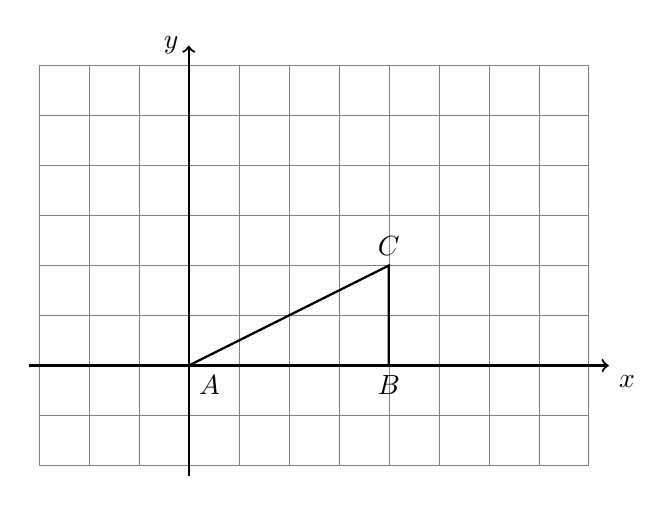
\begin{tikzpicture}[scale=.635]
       \draw [help lines] (-3,-2) grid (8,6);
       \draw [thick, ->] (-3.2,0) -- (8.4,0) node [below right] {$x$};
       \draw [thick, ->] (0,-2.2)--(0,6.4) node [left] {$y$};
       \draw [thick] (0,0)node[below right]{$A$}--
        (4,0)node[below]{$B$}--
          (4,2)node[above]{$C$}--cycle;
     \end{tikzpicture}
\vspace{0.5cm}

     \item Express each value to \emph{the nearest tenth}.  \vspace{0.5cm}
       \begin{multicols}{2}
         \begin{enumerate}
           \item $\tan 76^\circ = $ \vspace{0.5cm}
           \item $\cos 36^\circ =$
           \item $\tan 14^\circ = $ \vspace{0.5cm}
           \item $\sin 44^\circ =$
         \end{enumerate}
       \end{multicols}

     \item $\triangle ABC$ has sides of length $BC=6$, $AC=8$, and $AB=10$ as shown.\\[0.25cm] Use the Pythagorean theorem to show that $\triangle ABC$ is a right triangle with $m\angle C=90^\circ$. \vspace{4cm}
     \begin{multicols}{2}
         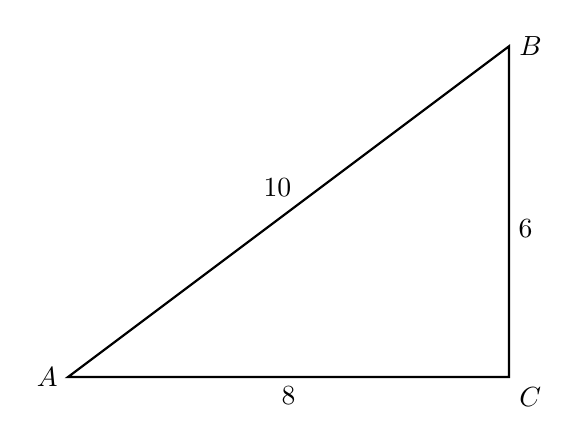
\begin{tikzpicture}[scale=0.7]
           \draw [thick]
           (0,0)node[left]{$A$}--
           (8,0)node[below right]{$C$}--
           (8,6)node[right]{$B$}--cycle;
           \node at (4,0)[below]{$8$};
           \node at (8,2.7)[right]{$6$};
           \node at (3.8,3.1)[above]{$10$};
         \end{tikzpicture}

         \begin{enumerate}
         \item Find $\tan A =$ \vspace{0.75cm}
         \item Find $\cos A =$ \vspace{0.75cm}

       \end{enumerate}
   \end{multicols}


  \newpage
\subsubsection*{Early finishers: Construction for project due Friday}

  Using a compass and straightedge, construct the line of reflection over which triangle $ABC$ reflects onto triangle $A'B'C'$. (Leave all construction marks.) \vspace{4cm}
      \begin{center}
      \begin{tikzpicture}[scale=1.5]
        %\draw [thick, <->] (-7.4,0) -- (10.4,0) node [right] {$x$};
        %\draw [thick, <->] (0,-6.4)--(0,10.4) node [above] {$y$};

        \draw [thick]
        (5,-1) node[below left] {$A$}--
        (6,3) node[right] {$B$}--
        (3,-1) node[below left] {$C$}--cycle;

        \draw [thick]
        (-1,5) node[left] {$A'$}--
        (3,6) node[above] {$B'$}--
        (-1,3) node[below left] {$C'$}--cycle;

      \end{tikzpicture}
    \end{center}

\end{enumerate}
\end{document}
